\section{考察}
実験で得られたデータからははっきりと波うつパターンが見て取れる。この章ではその波模様をいくつかの要素に分解し、それぞれについて理論的に説明できるかどうかを考えてゆく。私たちは望んだ干渉の結果を見ることができたのか。

\subsection{波模様の分解}

\ref{Resonance_sec}章で述べたように、干渉パターンは最も一般的には、共鳴からのずれを表すパラメータ$\epsilon$と中性子の速度$v$に依存した係数$N_1,N_2,N_3$を用いて
\begin{equation}
I=N_1-N_2\cos\left(\frac{2}{v}(\omega d'-\epsilon L')\right) -N_3\sin\left(\frac{2}{v}(\omega d'-\epsilon L')\right) \label{Discussion_theory_ippan}
\end{equation}
と表せる。ここで$\omega$は位相シフタコイルの磁場$B_p$を用いて$\omega=|\mu_n|B_p$と表される量であり、$d',L'$はそれぞれ位相シフタコイルの幅、2つのスピンフリッパー間距離である。さらに$N_4=\sqrt{N_2^2+N_3^2}$として
\begin{equation}
\cos \phi=\frac{N_2}{N_4}, \quad \sin \phi=\frac{N_3}{N_4}
\end{equation}
で$\phi$を定義すれば、干渉パターンは
\begin{equation}
I=N_1-N_4\cos\left(\frac{2}{v}(\omega d'-\epsilon L')-\phi\right)\label{Discussion_theory_ippan2}
\end{equation}
と書き直される。このように書くと実験データをフィッティングして得られる4つのパラメータと理論式を対応づけることができる。すなわち、実験で得られた波模様を位相シフタコイルに流した電流$I_p$に対して
\begin{equation}
I=D-A\cos(B\cdot I_p+C)
\end{equation}
という関数でフィッティングしたときの4つのパラメータ$A,B,C,D$は理論と
\begin{comment}
\renewcommand{\arraystretch}{1.5}
\begin{equation}
\begin{array}{l}
A \leftrightarrow N_4\\
B \leftrightarrow \dfrac{2\omega d'}{v(-I_p)}\\
C \leftrightarrow \dfrac{2\epsilon L'}{v} +\phi \\
D \leftrightarrow N_1
\end{array}
\end{equation}
\renewcommand{\arraystretch}{1}
\end{comment}
\begin{align}
A \leftrightarrow N_4&&B \leftrightarrow \dfrac{2\omega d'}{v(-I_p)}&&C \leftrightarrow \dfrac{2\epsilon L'}{v} +\phi&&D \leftrightarrow N_1
\end{align}
と対応づくことがわかる。なお、$I_p$は鉛直下向きに磁場が発生する向きを正としたため、$B,C$については理論式(\ref{Discussion_theory_ippan})のコサインの中身にマイナスをかけて対応づけておく。

なお、実験で得られたデータはある波長領域について積分したものであるため、ひとつの波長に対して定められた理論式(\ref{Discussion_theory_ippan})とは厳密には対応づかない。しかし十分狭い波長領域で見れば、近似的に領域の中心の波長に対する理論式と実験値を対応づけることができる。このことの詳しい議論は後で行う。

この節の要は、単に実験と理論を対応づけたということではなく、波模様というあいまいな概念を輪郭の明確な4つの要素に分解したことにある。これから4つの要素それぞれについて個別に考えてゆく。

\subsection{$B$}
\paragraph{パラメータ$B$の意味}
$B$には干渉という現象のエッセンスが凝縮されている。上では干渉パターンの最も一般的な形を見たが、逆に最も特殊な場合を見てみよう。それは共鳴条件()が満たされている中で、$\pi/2$フリップ条件()を満たす速度の中性子を対象とした場合である。そのときは$N_1=1/2,N_2=1/2,N_3=0,\epsilon=0$であるから、干渉パターンは
\begin{equation}
I=\frac{1}{2}\left(1-\cos\frac{2\omega d'}{v}\right) \label{Discussion_theory_simple}
\end{equation}
となる。このように、非常にシンプルな場合を考えてもスピン上下の位相差を表す$B$の部分の形は変わらない。そのような意味で$B$は干渉の本質を担っている。

\paragraph{理論からのアプローチ}
理論的には$B$は$2\omega d'/v(-I_p)$と書かれるが、$\omega \propto -I_p$であって、具体的に書けば
\begin{align}
\omega d'=\frac{|\mu_n|B_p d'}{\hbar}=\frac{(-I_p)|\mu_n| b_p d'}{\hbar}
\end{align}
となる。ここで$b_p$は位相シフタコイルに1Aの電流を流したときに発生する磁束密度。なおこの章では実験値と理論値を比較する必要からSI単位系を用い、$\hbar$も明記する。さらに位相シフタコイルによる磁場は空間的に一様ではないため、実際は粒子の軌道に沿った積分で表す必要がある:
\begin{equation}
b_p d' \rightarrow \int b_p(x) dx
\end{equation}

次の図\ref{Discussion_fig_PhaseShifterSimulation}は位相シフタコイルに1Aの電流を流したときの磁場分布シミュレーション結果である。%またシフタコイルの中心($y=z=0$)を通ったときの$x$軸に沿っての磁場分布を図\ref{Discussion_fig_PSS_danmen}に表す。
このシミュレーションを用いて$\int b_p(x) dx$を計算すると、シフタコイルの中心($y=z=0$)を通ったときの積分値は
\begin{equation}
\int b_p(x) dx =2.75 \times 10^{-5} \mathrm{T\cdot m/A}
\end{equation}
となった。なお積分範囲は実際の配置と図\ref{Discussion_fig_PSS_danmen}より、$-20$cmから$20$cmとした。また粒子の経路が$y$方向や$z$方向にずれたときの積分値は図\ref{Discussion_fig_PSS_zure}のようになった。ビームの幅は20mm程度であるから、中性子の経路による積分値のずれは1\%程度に抑えられると考えられる。そこで今後の解析には中心での値を用いることにする。
\begin{figure}[h]
\centering
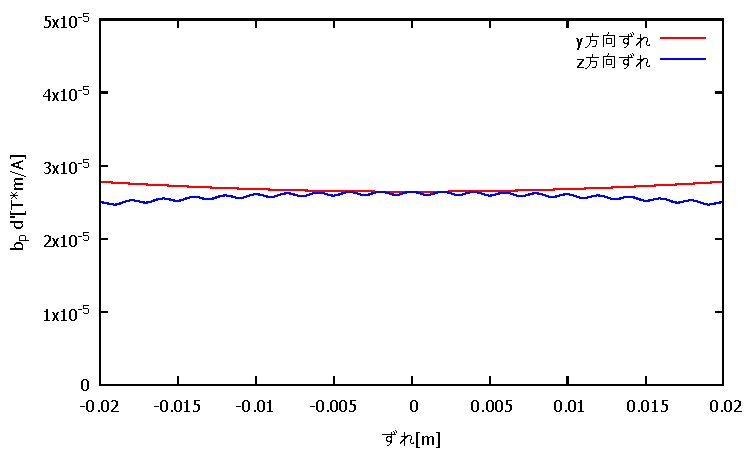
\includegraphics[width=9cm]{discussion/B/bd.pdf}
\caption{$y,z$方向のずれによる影響} \label{Discussion_fig_PSS_zure}
\vspace{-5mm}
\end{figure}

ゆえに$B$の理論値は
\begin{equation}
\frac{2\omega d'}{v(-I_p)}=2\frac{|\mu_n|\int b_p dx}{\hbar v}=2\frac{|\mu_n|\int b_p dx}{\hbar}\frac{m}{h}\lambda=1.27 \cdot \lambda \ [1/A] \label{Discussion_theory_B}
\end{equation}
となる。ただし$\lambda$[\AA]は中性子の波長。 

\begin{figure}[H]
%\begin{minipage}{0.5\hsize}
\begin{center}
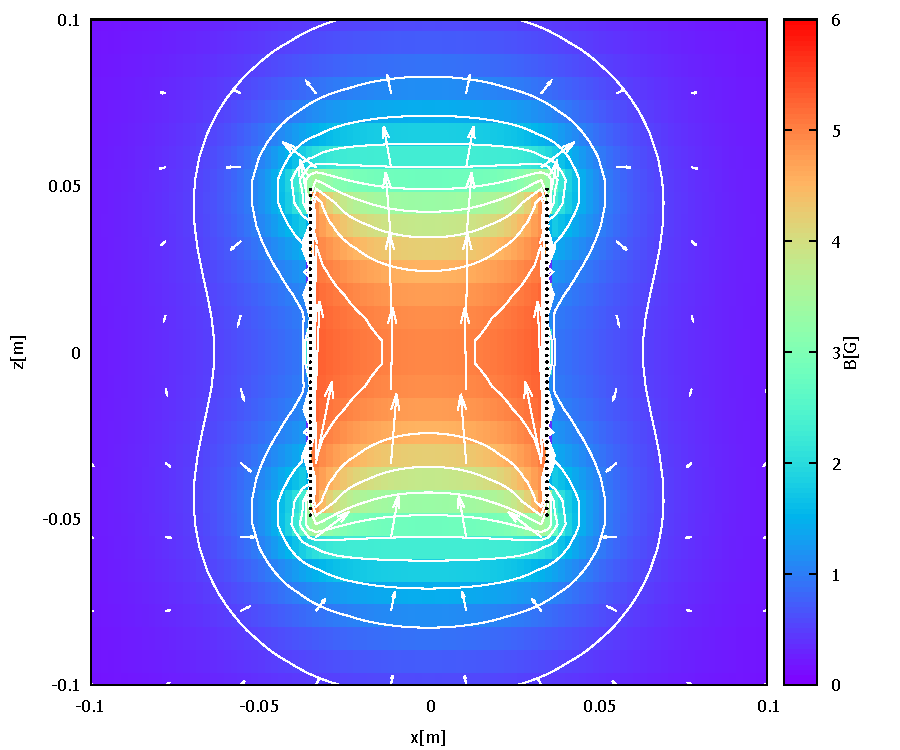
\includegraphics[width=9cm]{discussion/B/coil11_image1.pdf}
\vspace{-1mm}
\subcaption{横から}
\vspace{-3mm}
%\end{minipage}
%\begin{minipage}{0.5\hsize}
%\centering
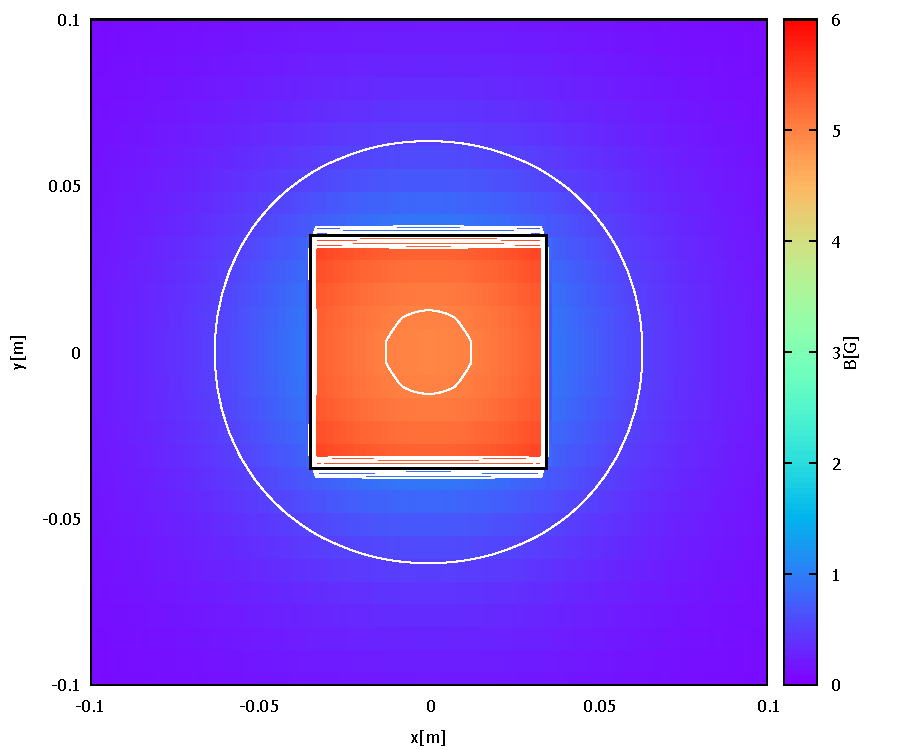
\includegraphics[width=9cm]{discussion/B/coil11_image2.pdf}
\vspace{-1mm}
\subcaption{上から}
\vspace{-3mm}
%\end{minipage}\\
%\begin{center}
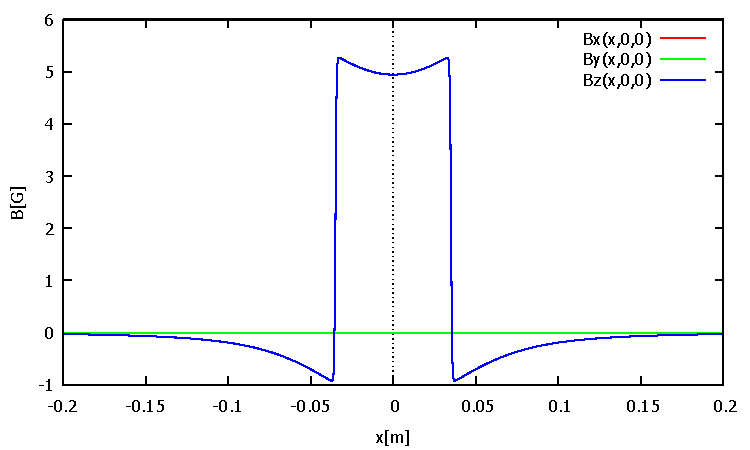
\includegraphics[width=9cm]{discussion/B/coil11_danmen1.pdf}
\vspace{-1mm}
\subcaption{中心($y=z=0$)を通ったとき}
\vspace{-3mm}
\end{center}
%\end{center}
\caption{位相シフタコイル磁場分布シミュレーション} \label{Discussion_fig_PhaseShifterSimulation}
%\vspace{-1cm}
\end{figure}

\paragraph{実験結果・解析}
以下の表\ref{Discussion_tbl_B}に波長領域$\lambda \pm 0.07 \AA$における実験データから得られた$B$の値と式(\ref{Discussion_theory_B})から得られる理論値を示す。なお理論値には中性子の経路による誤差1\% が含まれるとした。また表\ref{Discussion_tbl_B}の結果を図\ref{Discussion_fig_B}に表す。図、表からわかるように全ての波長領域でパラメータ$B$の実験値と理論値はよく一致しており、多くの波長において誤差の範囲で一致している。

\begin{figure}[h]
\begin{minipage}{0.35\hsize}
\centering
\makeatletter
\def\@captype{table}
\makeatother
\caption{各波長領域におけるパラメータ$B$の実験値と理論値} \label{Discussion_tbl_B}
\begin{tabular}{lll}
$\lambda$[\AA] &  $B(実験)$ &   理論値 \\ \hline
3.06  & 4.18  $\pm$ 0.05  & 3.90  $\pm$ 0.04  \\
3.21  & 4.14  $\pm$ 0.05  & 4.08  $\pm$ 0.04  \\
3.35  & 4.32  $\pm$ 0.05  & 4.27  $\pm$ 0.04  \\
3.42  & 4.42  $\pm$ 0.04  & 4.36  $\pm$ 0.04  \\
3.50  & 4.52  $\pm$ 0.05  & 4.45  $\pm$ 0.04  \\
3.56  & 4.63  $\pm$ 0.07  & 4.54  $\pm$ 0.05  \\
3.66  & 4.74  $\pm$ 0.07  & 4.66  $\pm$ 0.05  \\
3.75  & 4.77  $\pm$ 0.09  & 4.78  $\pm$ 0.05  \\
3.86  & 5.09  $\pm$ 0.09  & 4.91  $\pm$ 0.05  \\
4.00  & 5.15  $\pm$ 0.08  & 5.10  $\pm$ 0.05  \\
4.15  & 5.16  $\pm$ 0.18  & 5.28  $\pm$ 0.05  \\
4.29  & 3.36  $\pm$ 0.17  & 5.47  $\pm$ 0.05  \\ \hline
\end{tabular}
\end{minipage}
\begin{minipage}{0.65\hsize}
\centering
\vspace{2.5cm}
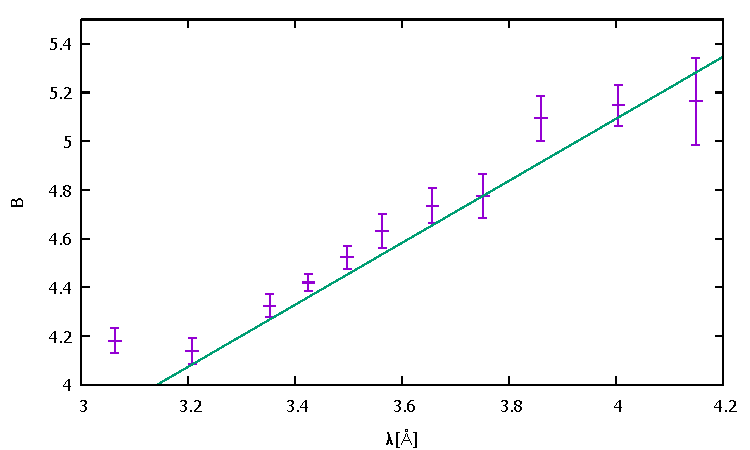
\includegraphics[width=10cm]{discussion/B/B_F.pdf}
\caption{各波長領域に対する$B$} \label{Discussion_fig_B}
\end{minipage}
\end{figure}

\paragraph{結論}
パラメータ$B$こそスピン干渉の本質であり、それが干渉のみられた全ての波長領域で理論値とよく一致したということは、私たちが望みのものを手に入れたということを示唆している。目的は果たされた。

\subsection{$C$}
\paragraph{パラメータ$C$の意味}
干渉においてパラメータ$B$の次に重要な意味をもつパラメータは$C$であろう。最もシンプルな場合(\ref{Discussion_theory_simple})を考えると、理論的にはパラメータ$C$に対応する位相のシフトは入ってこなかった:
\begin{equation}
I=\frac{1}{2}\left(1-\cos\frac{2\omega d'}{v}\right)
\end{equation}
$C$の対応物$2\epsilon L'/v +\phi$は、どちらの項も$\epsilon=0$のときゼロとなるためである。すなわちパラメータ$C$は共鳴からのずれに依存する。パラメータ$C$を分析することで、共鳴からのずれを知ることができる。

\paragraph{理論からのアプローチ}
理論的には$C$は$2\epsilon L'/v +\phi$に対応し、$\cos\phi=N_2/N_4,\sin\phi=N_3/N_4$であった。\ref{Resonance_sec}章より
\begin{align}
&N_2 = 2\left(\frac{\omega_r}{\omega_A}\right)^2\sin^2\frac{\omega_A}{v}d \left(\cos^2 \frac{\omega_A}{v}d -\left(\frac{\epsilon}{\omega_A}\right)^2 \sin^2 \frac{\omega_A}{v}d\right) \\
&N_3 = 4\frac{\epsilon}{\omega_A} \left(\frac{\omega_r}{\omega_A}\right)^2\sin^3\frac{\omega_A}{v}d \cos \frac{\omega_A}{v}d
\end{align}
であるから$N_4$は
\begin{equation}
N_4=\sqrt{N_2^2+N_3^2}=2\left(\frac{\omega_r}{\omega_A}\right)^2\sin^2\frac{\omega_A}{v}d \left(\cos^2\frac{\omega_A}{v}d+\left(\frac{\epsilon}{\omega_A}\right)^2\sin^2\frac{\omega_A}{v}d\right)
\end{equation}
と書ける。ここで$\omega_A=\sqrt{\epsilon^2+\omega_r^2}$であり、$d$はフリッパーの幅である。よって
\begin{align}
\cos\phi&=\frac{\cos^2 \frac{\omega_A}{v}d -\left(\frac{\epsilon}{\omega_A}\right)^2 \sin^2 \frac{\omega_A}{v}d}{\cos^2\frac{\omega_A}{v}d+\left(\frac{\epsilon}{\omega_A}\right)^2\sin^2\frac{\omega_A}{v}d} \\
\sin\phi&=\frac{2\frac{\epsilon}{\omega_A}\sin\frac{\omega_A}{v}d \cos \frac{\omega_A}{v}d}{\cos^2\frac{\omega_A}{v}d+\left(\frac{\epsilon}{\omega_A}\right)^2\sin^2\frac{\omega_A}{v}d}
\end{align}
であり、確かに$\epsilon=0$のとき$\phi=0$となる。次の図\ref{Discussion_fig_phi}に$\epsilon/\omega_z=0,0.1,0.3,0.5,1.0$のときの中性子の波長$\lambda$に対する$\phi$の理論値を表す。ただし$\omega_r/\omega_z=0.25,B_z=12.8\,\mathrm{G}$とした。
\begin{figure}[h]
\centering
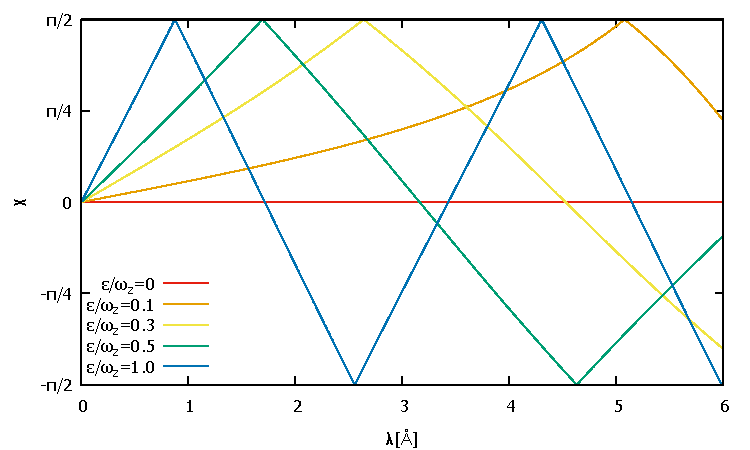
\includegraphics[width=10cm]{discussion/C/chi.pdf}
\caption{中性子の波長$\lambda$に対する$\phi$} \label{Discussion_fig_phi}
\end{figure}

これを実験値と比べるためにはもう一工夫必要となる。理論では上流と下流のスピンフリッパーで$\omega_r$の値は等しいとしていた。しかし、実際に測定データから得られた$\omega_r$は上流と下流で異なっていた(\ref{Resonance_sec}章参照)。%上流、下流フリッパーの$\omega_r$をそれぞれ$\omega_{r1},\omega_{r2}$とすると$\omega_r/2\pi=8.7\pm0.1\,\mathrm{kHz},
そこで上流、下流フリッパーの$\omega_r$をそれぞれ$\omega_{r1},\omega_{r2}$として、2つのフリッパーで$\omega_r$が異なる場合も含めた干渉パターンの式を求めると、式の形は$\omega_r$が等しい場合(\ref{Discussion_theory_ippan})と同じで、係数が
\begin{align}
&N_1 = \left(\cos^2 \frac{\omega_{A1}}{v}d +\left(\frac{\epsilon}{\omega_{A1}}\right)^2\sin^2 \frac{\omega_{A1}}{v}d\right)\left(\cos^2 \frac{\omega_{A2}}{v}d+\left(\frac{\epsilon}{\omega_{A2}}\right)^2 \sin^2 \frac{\omega_{A2}}{v}d\right)\\ \notag
&\hspace{7cm}+\left(\frac{\omega_{r1}}{\omega_{A1}}\right)^2\left(\frac{\omega_{r2}}{\omega_{A2}}\right)^2 \sin^2 \frac{\omega_{A1}}{v}d \sin^2 \frac{\omega_{A2}}{v}d\\
&N_2 = 2\frac{\omega_{r1}}{\omega_{A1}}\frac{\omega_{r2}}{\omega_{A2}}\sin\frac{\omega_{A1}}{v}d\sin\frac{\omega_{A2}}{v}d \left(\cos \frac{\omega_{A1}}{v}d\cos \frac{\omega_{A2}}{v}d -\frac{\epsilon}{\omega_{A1}}\frac{\epsilon}{\omega_{A2}} \sin \frac{\omega_{A1}}{v}d\sin \frac{\omega_{A2}}{v}d\right) \\
&N_3 = 2\frac{\omega_{r1}}{\omega_{A1}}\frac{\omega_{r2}}{\omega_{A2}}\sin\frac{\omega_{A1}}{v}d\sin\frac{\omega_{A2}}{v}d \left(\frac{\epsilon}{\omega_{A1}}\sin \frac{\omega_{A1}}{v}d\cos \frac{\omega_{A2}}{v}d +\frac{\epsilon}{\omega_{A2}} \sin \frac{\omega_{A1}}{v}d\cos \frac{\omega_{A2}}{v}d\right)
\end{align}\label{Discussion_theory_ippanippan}
となる。ここで$\omega_{Ai}=\sqrt{\epsilon^2+\omega_{ri}^2} \ (i=1,2)$である。これでパラメータ$C$について実験値と理論値を比較する準備が整った。

\paragraph{実験結果}
以下の表\ref{Discussion_tbl_C}に波長領域$\lambda \pm 0.07 \AA$における実験データから得られた$C$の値を示し、中心波長$\lambda$と$C$の関係を図\ref{Discussion_fig_C}に表す。
\begin{figure}[h]
\begin{minipage}{0.35\hsize}
\centering
\makeatletter
\def\@captype{table}
\makeatother
\caption{各波長領域におけるパラメータ$C$の実験値} \label{Discussion_tbl_C}
\begin{tabular}{ll}
$\lambda$[\AA] &  $C(実験)$\\ \hline
3.06 	&	1.12 	$\pm$	0.09 \\
3.21 	&	1.61 	$\pm$	0.09 \\
3.35 	&	1.90 	$\pm$	0.07 \\
3.42 	&	2.04 	$\pm$	0.06 \\
3.50 	&	2.14 	$\pm$	0.08 \\
3.56 	&	2.27 	$\pm$	0.12 \\
3.66 	&	2.50 	$\pm$	0.12 \\
3.75 	&	2.52 	$\pm$	0.14 \\
3.86 	&	2.87 	$\pm$	0.16 \\
4.00 	&	3.12 	$\pm$	0.15 \\
4.15 	&	3.72 	$\pm$	0.31 \\
4.29 	&	3.76 	$\pm$	0.28 \\ \hline
\end{tabular}
\end{minipage}
\begin{minipage}{0.65\hsize}
\centering
\vspace{2.5cm}
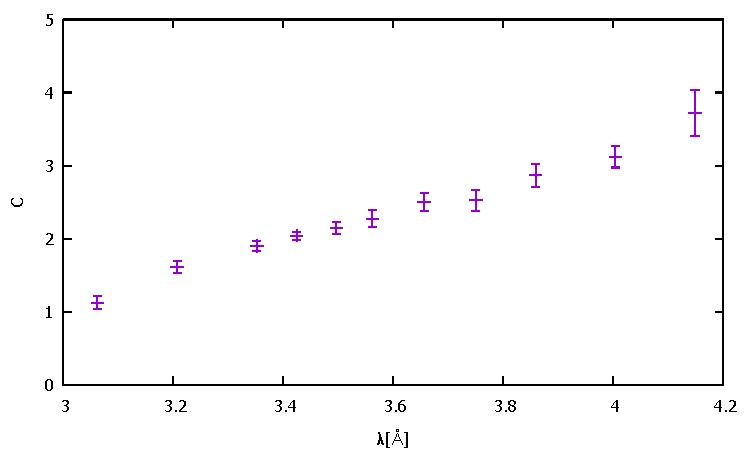
\includegraphics[width=10cm]{discussion/C/C_F.pdf}
\caption{中心波長$\lambda$と$C$の関係} \label{Discussion_fig_C}
\end{minipage}
\end{figure}

\paragraph{解析}
$\epsilon/\omega_z$をフィッティングパラメータとして実験値をフィッティングすることを考える。このときフィッティング関数は$2\epsilon L'/v +\phi$であるが、正確には$2n\pi$(n:整数)の不定性が存在する。そこでフィッティング関数として次の形を用い、$n=-3,-2,-1,0,1,2$の各場合についてフィッティングを行った。
\begin{equation}
2\epsilon L'/v +\phi+2n\pi
\end{equation}
なお、各種パラメータには実測と測定データから求めた次の値を用いた。
\begin{table}[h]
\centering
\caption{各種パラメータ}\label{Discussion_tbl_parameter}
\begin{tabular}{ccccc}
$\omega_{r1}/2\pi$[kHz]&$\omega_{r2}/2\pi$[kHz]&$\omega_{z}/2\pi$[kHz]&$d$[mm]&$L'$[mm]\\ \hline
4.4&4.8&18.7&30&273
\end{tabular}
\end{table}

次の表\ref{Discussion_tbl_Cfit}に各$n$におけるフィッティングの結果を示す。カイ二乗が最も小さくなった$n=-1$のときについてフィッティング結果を図\ref{Discussion_fig_Cfit}に表す。

\paragraph{結論}
パラメータ$C$は共鳴からのずれと関係づく。$\epsilon/\omega_z=0.131\pm0.001$とすると、干渉のみられた全ての波長領域でパラメータ$C$の実験値は理論値とよく一致した。すなわち今回の実験における共鳴からのずれは$\epsilon/\omega_z=0.131\pm0.001$程度であったと推測される。

\begin{table}[H]
\centering
\caption{$n=-3,-2,-1,0,1,2$に対するフィッティング結果}\label{Discussion_tbl_Cfit}
\begin{tabular}{ccc}
$n$&$\epsilon/\omega_z$&reduced $\chi^2$\\ \hline
$-3$	&$0.364 \pm0.004$ 	&56.8 \\
$-2$	&$0.237 \pm0.002$ 	&9.43 \\
$-1$	&$0.131 \pm0.001$ 	&2.16 \\
$0$	&$0.033 \pm0.002$ 	&14.1 \\
$1$	&$-0.066 \pm0.004$ 	&76.1 \\
$2$	&$-0.165 \pm0.006$ 	&182\\ \hline
\end{tabular}
\end{table}
\begin{figure}[h]
\centering
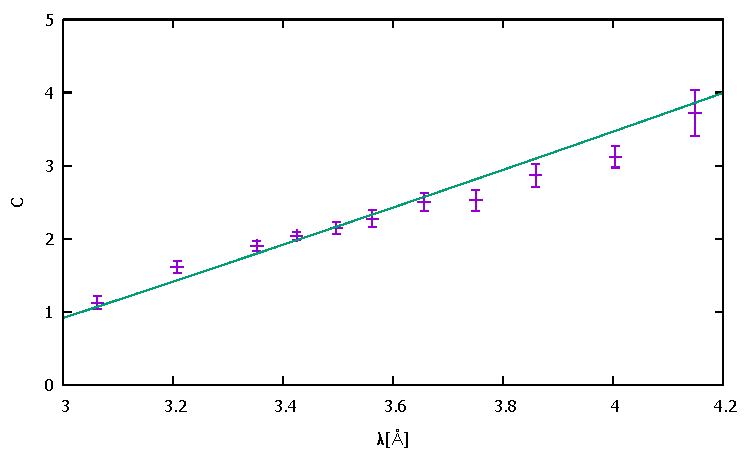
\includegraphics[width=10cm]{discussion/C/C_F_fit.pdf}
\caption{$n=-1$のときのフィッティング結果}\label{Discussion_fig_Cfit}
\end{figure}

\subsection{$D$}
\paragraph{パラメータ$D$の意味}
パラメータ$D$は干渉の波模様がどこを中心に振動しているかを表す。パラメータ$D$は波の位相ではなく波の高さに関係した量であるという点で、前述のパラメータ$B$や$C$と異なる。波の位相については粒子数の相対的な差から情報を得ることができるが、波の高さについては粒子数の絶対値が影響する。したがってパラメータ$D$からはパラメータ$B$,$C$からは知り得なかった粒子数の絶対値に関係した情報を得ることができる。

\paragraph{理論からのアプローチ}
理論的には$D$は$N_1$に対応する。2つのフリッパーで$\omega_r$が異なる場合も含めた最も一般的な$N_1$の表式は次の通りであった:
\begin{align}
&N_1 = \left(\cos^2 \frac{\omega_{A1}}{v}d +\left(\frac{\epsilon}{\omega_{A1}}\right)^2\sin^2 \frac{\omega_{A1}}{v}d\right)\left(\cos^2 \frac{\omega_{A2}}{v}d+\left(\frac{\epsilon}{\omega_{A2}}\right)^2 \sin^2 \frac{\omega_{A2}}{v}d\right)\\ \notag
&\hspace{7cm}+\left(\frac{\omega_{r1}}{\omega_{A1}}\right)^2\left(\frac{\omega_{r2}}{\omega_{A2}}\right)^2 \sin^2 \frac{\omega_{A1}}{v}d \sin^2 \frac{\omega_{A2}}{v}d
\end{align}
これを種々の$\epsilon/\omega_z$に対して波長を横軸として図示すると図\ref{Discussion_fig_N1}のようになる。各種パラメータには表\ref{Discussion_tbl_parameter}の値を用いた。
\begin{figure}[h]
\centering
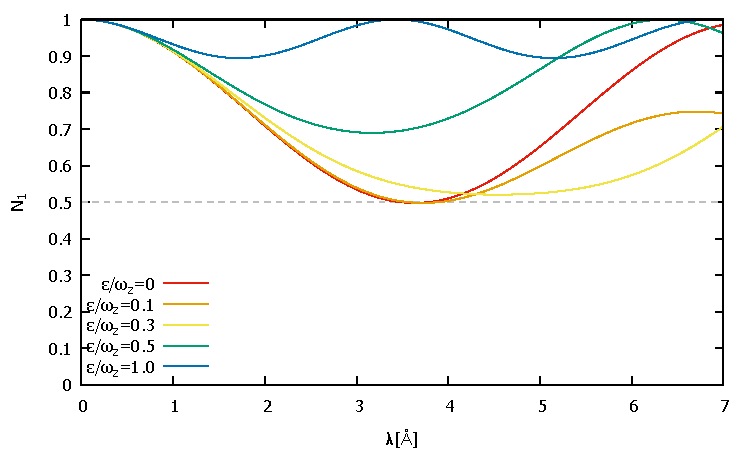
\includegraphics[width=10cm]{discussion/D/N1.pdf}
\caption{中性子の波長$\lambda$に対する$N_1$}\label{Discussion_fig_N1}
\end{figure}

\paragraph{実験結果}
以下の表\ref{Discussion_tbl_D}に波長領域$\lambda \pm 0.07 \AA$における実験データから得られた$D$の値を示し、中心波長$\lambda$と$D$の関係を図\ref{Discussion_fig_D}に表す。
\begin{figure}[H]
\begin{minipage}{0.35\hsize}
\centering
\makeatletter
\def\@captype{table}
\makeatother
\caption{各波長領域におけるパラメータ$D$の実験値} \label{Discussion_tbl_D}
\begin{tabular}{ll}
$\lambda$[\AA] &  $D(実験)$\\ \hline
3.06 	&	0.61 	$\pm$	0.05 	\\
3.21 	&	0.63 	$\pm$	0.05 	\\
3.35 	&	0.53 	$\pm$	0.04 	\\
3.42 	&	0.59 	$\pm$	0.05 	\\
3.50 	&	0.63 	$\pm$	0.05 	\\
3.56 	&	0.59 	$\pm$	0.05 	\\
3.66 	&	0.58 	$\pm$	0.05 	\\
3.75 	&	0.66 	$\pm$	0.06 	\\
3.86 	&	0.69 	$\pm$	0.07 	\\
4.00 	&	0.91 	$\pm$	0.10 	\\
4.15 	&	0.79 	$\pm$	0.09 	\\
4.29 	&	0.81 	$\pm$	0.09 	\\ \hline
\end{tabular}
\end{minipage}
\begin{minipage}{0.65\hsize}
\centering
\vspace{2.5cm}
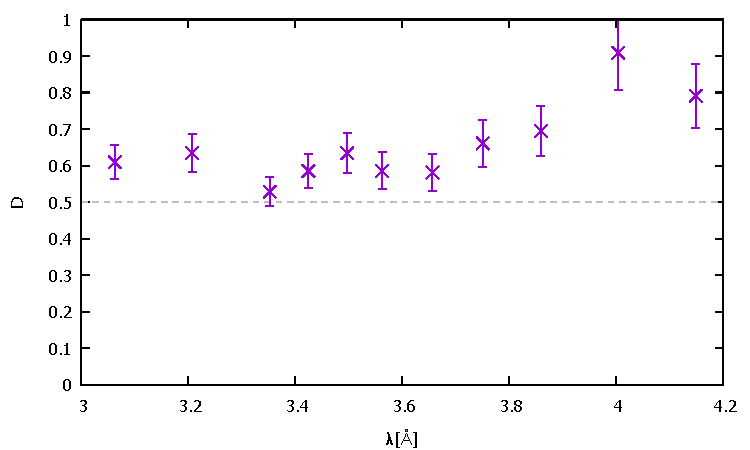
\includegraphics[width=10cm]{discussion/D/D_F.pdf}
\caption{中心波長$\lambda$と$D$の関係} \label{Discussion_fig_D}
\end{minipage}
\end{figure}

\paragraph{解析}
パラメータ$C$に対する考察の結果から$\epsilon/\omega_z=0.131$としたときの$D$の理論値を実験値と共に図\ref{Discussion_fig_D_N1}に表す。このときreduced$\chi^2=74/12=6.2$となり、理論値と実験値の一致はあまりよくない。全ての波長において実験値は理論値よりも上にずれている。これは粒子数の変動の中心が数の多い方へシフトしていることを意味しており、バックグラウンドの存在が示唆される。
\begin{figure}[h]
\centering
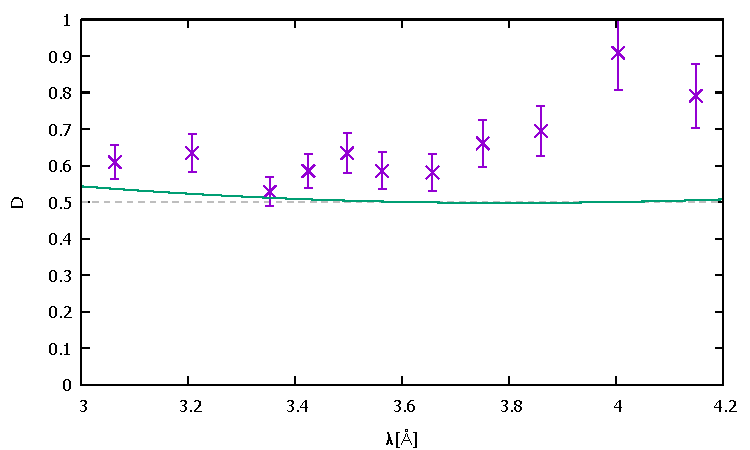
\includegraphics[width=10cm]{discussion/D/D_F_N1.pdf}
\caption{波長に対する$D$の実験値と$\epsilon/\omega_z=0.131$のときの理論値}
\end{figure}

\paragraph{結論}
パラメータ$D$は干渉波が振動する中心の高さを表し、パラメータ$B$や$C$からは知り得なかった粒子数の絶対値に関する情報を教えてくれる。$D$の実験値が理論値と比べて大きくなっていることはバックグラウンドの存在を示唆している。バックグラウンドに関する詳しい議論は後にまわす。

\subsection{$A$}
\paragraph{パラメータ$A$の意味}
パラメータ$A$は干渉の波模様の振幅を表す。パラメータ$A$は$D$と同様に波の高さに関係した量であり、絶対的な粒子数に関する情報を持つ。一方で位相のずれた波が重なるとうなりが生じて振幅は変化する。その意味でパラメータ$A$は位相に関する情報も持っているといえる。

\paragraph{理論からのアプローチ}
理論的には$A$は$N_4$に対応する。その具体的な表式は式(\ref{Discussion_theory_ippanippan})より
\begin{align}
N_4&=\sqrt{N_2^2+N_3^2} \notag \\
&=2\frac{\omega_{r1}}{\omega_{A1}}\frac{\omega_{r2}}{\omega_{A2}}\sin\frac{\omega_{A1}}{v}d\sin\frac{\omega_{A2}}{v}d\sqrt{\left(\cos^2 \frac{\omega_{A1}}{v}d +\left(\frac{\epsilon}{\omega_{A1}}\right)^2\sin^2 \frac{\omega_{A1}}{v}d\right)\left(\cos^2 \frac{\omega_{A2}}{v}d+\left(\frac{\epsilon}{\omega_{A2}}\right)^2 \sin^2 \frac{\omega_{A2}}{v}d\right)}
\end{align}
である。これを種々の$\epsilon/\omega_z$に対して波長を横軸として図示すると図\ref{Discussion_fig_N4}のようになる。各種パラメータには表\ref{Discussion_tbl_parameter}の値を用いた。図\ref{Discussion_fig_N4}は波長に対する$N_1$を描いた図\ref{Discussion_fig_N1}を0.5を境に反転したように見える。実際、$\omega_{r1}=\omega_{r2}$のときは$N_1+N_4=1$が厳密になりたつ。つまり上流下流のスピンフリッパーで$\omega_r$が等しいときは共鳴のいかんに関わらず常に干渉の波の頂上は1に達する(図\ref{Resonance_fig_interference}参照)。
\begin{figure}[H]
\centering
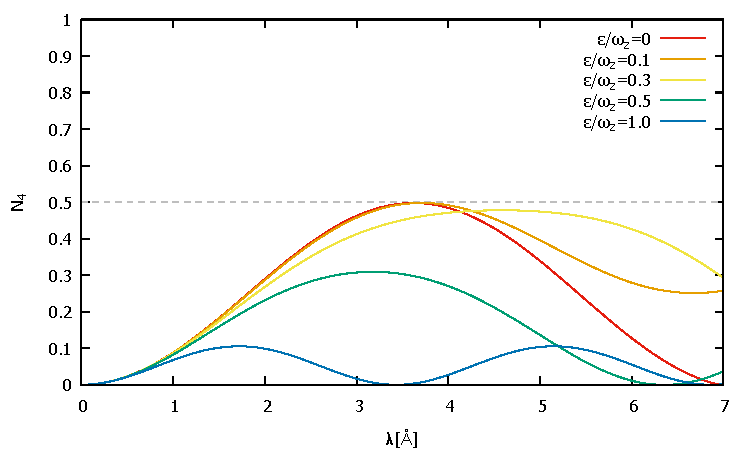
\includegraphics[width=10cm]{discussion/A/N4.pdf}
\caption{中性子の波長$\lambda$に対する$N_4$}\label{Discussion_fig_N4}
\end{figure}

\paragraph{実験結果}
以下の表\ref{Discussion_tbl_A}に波長領域$\lambda \pm 0.07 \AA$における実験データから得られた$A$の値を示し、中心波長$\lambda$と$A$の関係を図\ref{Discussion_fig_A}に表す。
\begin{figure}[H]
\begin{minipage}{0.35\hsize}
\centering
\makeatletter
\def\@captype{table}
\makeatother
\caption{各波長領域におけるパラメータ$A$の実験値} \label{Discussion_tbl_A}
\begin{tabular}{ll}
$\lambda$[\AA] &  $A(実験)$\\ \hline
3.06 	&	0.21 	$\pm$	0.02 	\\
3.21 	&	0.27 	$\pm$	0.03 	\\
3.35 	&	0.25 	$\pm$	0.02 	\\
3.42 	&	0.28 	$\pm$	0.03 	\\
3.50 	&	0.30 	$\pm$	0.03 	\\
3.56 	&	0.24 	$\pm$	0.03 	\\
3.66 	&	0.20 	$\pm$	0.03 	\\
3.75 	&	0.24 	$\pm$	0.04 	\\
3.86 	&	0.17 	$\pm$	0.03 	\\
4.00 	&	0.21 	$\pm$	0.04 	\\
4.15 	&	0.15 	$\pm$	0.04 	\\
4.29 	&	0.11 	$\pm$	0.03 	\\ \hline
\end{tabular}
\end{minipage}
\begin{minipage}{0.65\hsize}
\centering
\vspace{2.5cm}
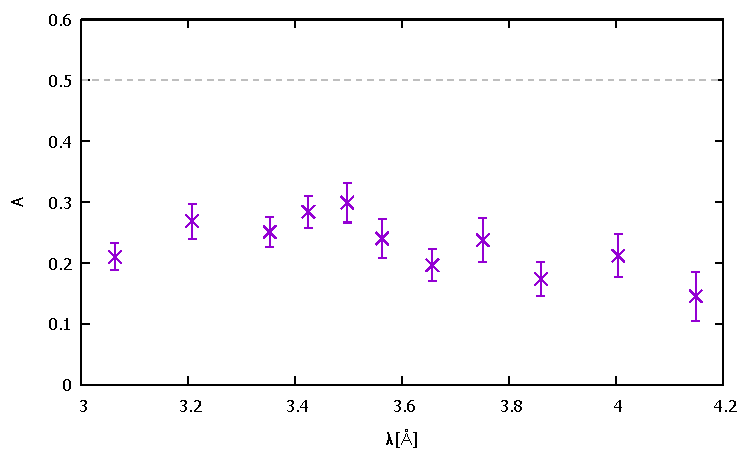
\includegraphics[width=10cm]{discussion/A/A_F.pdf}
\caption{中心波長$\lambda$と$A$の関係} \label{Discussion_fig_A}
\end{minipage}
\end{figure}

\paragraph{解析}
パラメータ$C$に対する考察の結果から$\epsilon/\omega_z=0.131$としたときの$A$の理論値を実験値と共に図\ref{Discussion_fig_A_N4}に表す。このときreduced$\chi^2=1041/12=87$となり、理論値と実験値の一致は悪い。全ての波長において実験値は理論値よりも大きく下にずれている。これは干渉波の振幅が理論の予想より小さいことを意味する。この原因として、バックグラウンドによって波の高さの振動中心が上へずれたことと、位相のずれた波が重ね合わさり振幅が減衰したことの2つが考えられる。
\begin{figure}[h]
\centering
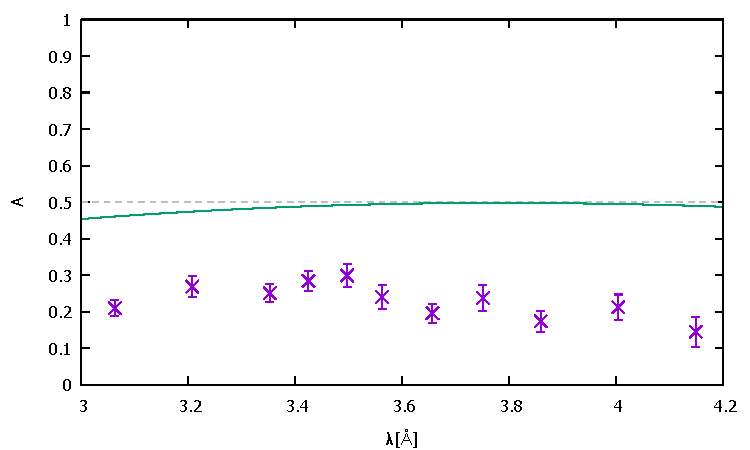
\includegraphics[width=10cm]{discussion/A/A_F_N4.pdf}
\caption{波長に対する$D$の実験値と$\epsilon/\omega_z=0.131$のときの理論値}
\end{figure}

\paragraph{結論}
パラメータ$A$は干渉波の振幅を表し、波の高さと位相の両方に依存する。干渉をみる波長領域の中心波長に対する理論値と実験値は一致せず、実験値は理論値の半分程度となった。観測粒子数にあるバックグラウンドが含まれており、粒子数の変動の中心が数の多い方へずれたこと、実験で得られたデータはある波長領域について観測粒子数を積分したものであり、位相のずれた波が重ね合わさることで振幅が減衰したことが原因として考えられる。






